\chapter{A reprodução sexuada}\label{ch:g8:sexual-reproduction}

O canto dos sapos em maio, as \omterm{def:g3:flowers-fruits-seeds:parts}{flores} da cerejeira em abril, o berro do
cervo no outono, um girassol virando a face cheia de \omterm{def:g3:flowers-fruits-seeds:parts}{flores} para as
abelhas: por todo o mundo vivo, uma \omterm{prop:g3:balanced-diet:jobs}{energia} enorme é gasta num único
projeto --- a geração seguinte. Os anos anteriores juntaram as peças
(\cref{ch:g4:animal-reproduction},
\cref{ch:g5:flower-to-fruit}); este ano as monta numa teoria só e faz
a pergunta mais afiada: por que \emph{dois} pais, afinal?

\begin{omfigure}
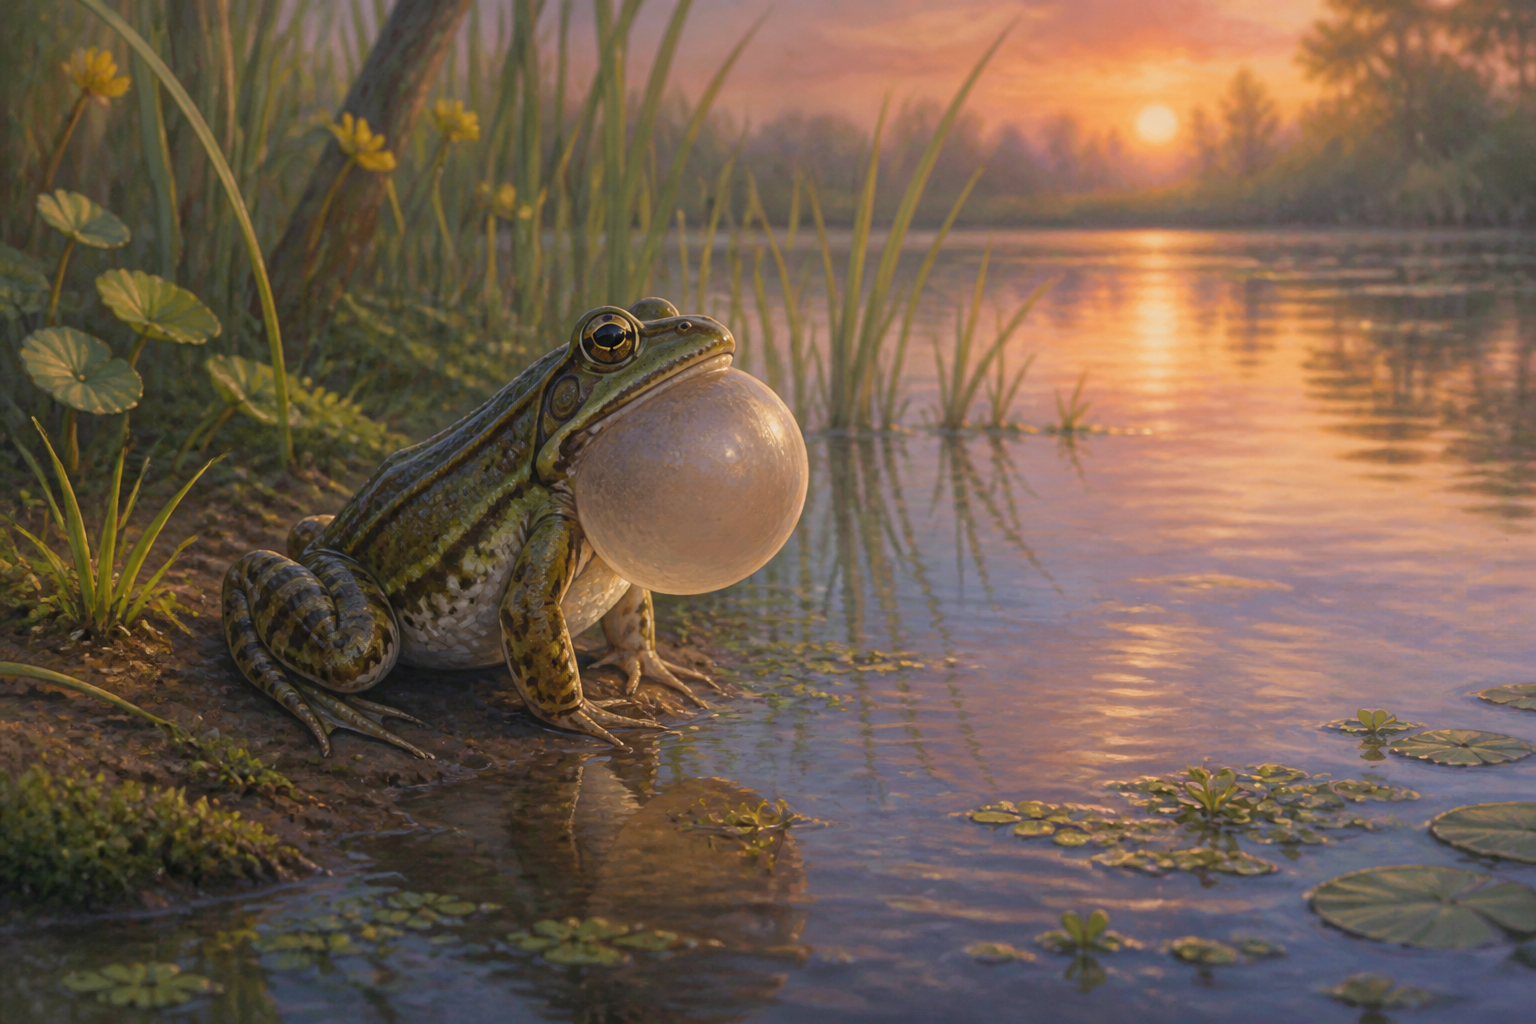
\includegraphics[width=0.6\linewidth]{images/book1/ai/g8-frog-chorus.png}

{\small \omterm{prop:g3:balanced-diet:jobs}{Energia} enorme para um projeto só: o saco vocal inflado do
\omterm{def:g4:animal-reproduction:sexual}{macho}, convocando a lagoa para o encontro dos \omterm{def:g8:sexual-reproduction:gametes}{gametas}.}
\end{omfigure}

\section{Um mecanismo em todo o mundo vivo}

\begin{definition}[Gametas]\label{def:g8:sexual-reproduction:gametes}
As \omterm{def:g5:first-look-at-cells:cell}{células} reprodutoras da
\cref{def:g4:animal-reproduction:sexual} recebem o nome geral de
\emph{gametas}\index{gameta}: o gameta masculino (o \omterm{def:g4:animal-reproduction:sexual}{espermatozoide} nos
\omterm{def:g1:animals-around-us:animal}{animais}, a \omterm{def:g5:first-look-at-cells:cell}{célula} do grão de \omterm{def:g3:flowers-fruits-seeds:parts}{pólen} nas \omterm{def:g1:plants-around-us:plant}{plantas} com \omterm{def:g3:flowers-fruits-seeds:parts}{flor}) e o gameta
feminino (a \omterm{def:g4:animal-reproduction:sexual}{célula reprodutora feminina}, no ovário ou no óvulo). Os
gametas são \omterm{def:g5:first-look-at-cells:cell}{células} únicas (\cref{ch:g5:first-look-at-cells}), e cada
um é metade de um começo: sozinho, um gameta morre; juntos, dois fazem
uma vida.
\end{definition}

\begin{proposition}[O núcleo invariável]\label{prop:g8:sexual-reproduction:core}
Onde quer que a \omterm{def:g4:animal-reproduction:sexual}{reprodução sexuada} aconteça --- peixe ou pinheiro,
caracol ou ser humano --- o \omterm{def:g6:cell-unit-of-life:parts}{núcleo} é invariável:
\begin{enumerate}
  \item dois pais produzem \omterm{def:g8:sexual-reproduction:gametes}{gametas}, masculino e feminino;
  \item a \emph{\omterm{def:g5:flower-to-fruit:steps}{fecundação}}: um \omterm{def:g8:sexual-reproduction:gametes}{gameta} masculino se junta a um \omterm{def:g8:sexual-reproduction:gametes}{gameta}
        feminino, formando uma única \omterm{def:g5:first-look-at-cells:cell}{célula} nova --- a
        \emph{\omterm{def:g4:animal-reproduction:sexual}{célula reprodutora feminina} fecundada}, ou
        \emph{zigoto}\index{zigoto};
  \item o \omterm{prop:g8:sexual-reproduction:core}{zigoto} se divide e se divide
        (\cref{prop:g5:first-look-at-cells:growth}), construindo um
        novo indivíduo que carrega algo dos \emph{dois} pais
        (\cref{rem:g4:animal-reproduction:mix}).
\end{enumerate}
Em volta desse \omterm{def:g6:cell-unit-of-life:parts}{núcleo}, todo o resto é variação: onde os \omterm{def:g8:sexual-reproduction:gametes}{gametas} se
encontram, quantos são, quem cuida dos filhotes.
\end{proposition}
\admitted

\begin{example}[As variações, classificadas]\label{ex:g8:sexual-reproduction:variations}
A coleção antiga se arquiva direitinho sob o \omterm{def:g6:cell-unit-of-life:parts}{núcleo}. \omterm{def:g5:flower-to-fruit:steps}{Fecundação}
externa contra interna
(\cref{prop:g4:animal-reproduction:where}): o lugar do encontro.
\omterm{def:g4:animal-reproduction:ovivivi}{Ovíparo} contra \omterm{def:g4:animal-reproduction:ovivivi}{vivíparo}
(\cref{def:g4:animal-reproduction:ovivivi}): a hospedagem do \omterm{prop:g8:sexual-reproduction:core}{zigoto}.
Os milhões do bacalhau contra o filhote único da elefanta
(\cref{prop:g4:animal-reproduction:strategies}): o balanço dos
números. \omterm{def:g5:flower-to-fruit:steps}{Polinização} por abelha ou pelo vento
(\cref{def:g5:flower-to-fruit:steps}): o serviço de viagem do \omterm{def:g8:sexual-reproduction:gametes}{gameta}
masculino. Um mecanismo, um catálogo de ajustes.
\end{example}

\begin{remark}[As plantas rodam o mesmo núcleo]\label{rem:g8:sexual-reproduction:plants}
Ponha o \cref{ch:g5:flower-to-fruit} ao lado do
\cref{ch:g4:animal-reproduction} e a correspondência é exata: os
\omterm{def:g3:flowers-fruits-seeds:parts}{estames} e o \omterm{def:g3:flowers-fruits-seeds:parts}{pistilo} produzem os \omterm{def:g8:sexual-reproduction:gametes}{gametas}, o tubo polínico é o corredor
da \omterm{def:g5:flower-to-fruit:steps}{fecundação} interna, a \omterm{def:g2:from-seed-to-plant:seed}{semente} hospeda o \omterm{def:g5:human-reproduction:pregnancy}{embrião} da \omterm{def:g1:plants-around-us:plant}{planta} com o
lanche embalado dele
(\cref{def:g2:from-seed-to-plant:seed}). Só a \omterm{def:g4:plants-without-seeds:vegetative}{reprodução vegetativa}
(\cref{def:g4:plants-without-seeds:vegetative}) fica de fora --- um pai
só, sem \omterm{def:g8:sexual-reproduction:gametes}{gametas}, com cópias exatas: o contraste que deixa afiada a
pergunta da próxima seção.
\end{remark}

\section{Por que dois pais?}

\begin{proposition}[A reprodução sexuada embaralha]\label{prop:g8:sexual-reproduction:shuffle}
As cópias de morangueiro dos \omterm{ex:g4:plants-without-seeds:runner}{estolhos}
(\cref{rem:g4:plants-without-seeds:copy}) mostram o que um pai só
rende: mesmice. Dois pais rendem o oposto. Como todo \omterm{prop:g8:sexual-reproduction:core}{zigoto} combina um
\omterm{def:g8:sexual-reproduction:gametes}{gameta} de cada pai --- e, como um capítulo mais adiante vai mostrar,
nem dois \omterm{def:g8:sexual-reproduction:gametes}{gametas} de um mesmo pai carregam exatamente a mesma herança
--- a \omterm{def:g4:animal-reproduction:sexual}{reprodução sexuada} dá a cada filho uma \emph{combinação nova}. Os
irmãos diferem; nem duas \omterm{prop:g2:from-seed-to-plant:cycle}{plântulas} de uma mesma vagem são iguais; a
variedade dentro de cada \omterm{def:g5:biodiversity:species}{espécie}
(\cref{rem:g5:biodiversity:scales}) é, em boa parte, obra desse
embaralhamento.
\end{proposition}
\admitted

\begin{example}[As duas apostas do pomar]\label{ex:g8:sexual-reproduction:bets}
O pomar da \cref{rem:g4:plants-without-seeds:copy} joga os dois jogos
sabendo o que faz. Enxertos e \omterm{met:g4:plants-without-seeds:cutting}{estacas}: um pai só, cópias exatas da
árvore excelente --- e uma fraqueza compartilhada, então uma praga que
derruba uma pode derrubar todas. Caroços: dois pais, cada \omterm{prop:g2:from-seed-to-plant:cycle}{plântula} uma
combinação nova --- quase todas sem nada de especial, algumas piores,
uma rara melhor que qualquer um dos pais, e nenhuma igual à outra para
uma praga varrer. Copiar guarda o presente; embaralhar explora o
futuro.
\end{example}

\begin{remark}[A variedade é a reserva da espécie]\label{rem:g8:sexual-reproduction:reserve}
Por que o embaralhamento importa para além do pomar: a
\cref{prop:g5:biodiversity:web} mostrou teias absorvendo baques
graças à variedade de \omterm{def:g5:biodiversity:species}{espécies}; dentro de uma \omterm{def:g5:biodiversity:species}{espécie}, a variedade de
indivíduos faz o mesmo papel. Quando as \omterm{def:g6:exploring-our-environment:conditions}{condições} viram --- uma doença
nova, um inverno mais duro --- uma \omterm{def:g5:biodiversity:species}{espécie} variada tem mais chance de
ter alguém adequado às novas regras. O que isso sugere sobre a
história da vida, o \cref{ch:g9:how-species-change} vai tornar
explícito; aqui, repare só que a \omterm{def:g4:animal-reproduction:sexual}{reprodução sexuada} é o que mantém a
reserva abastecida.
\end{remark}

\section{Ler a reprodução de qualquer espécie}

\begin{method}[O dossiê da reprodução]\label{met:g8:sexual-reproduction:dossier}
Para qualquer \omterm{def:g5:biodiversity:species}{espécie}, monte:
\begin{enumerate}
  \item \omterm{def:g8:sexual-reproduction:gametes}{gametas}: quem produz qual, e onde;
  \item encontro: \omterm{def:g5:flower-to-fruit:steps}{fecundação} externa ou interna, e o serviço de
        viagem (água, \omterm{prop:g4:animal-reproduction:where}{acasalamento}, polinizador, vento);
  \item hospedagem: \omterm{def:g2:animals-grow-up:born}{ovos} postos ou filhotes carregados; com que
        provisões;
  \item números e cuidado: a posição na linha das estratégias
        (\cref{prop:g4:animal-reproduction:strategies});
  \item estação: quando, e regulada por quê --- pergunta do próximo
        capítulo.
\end{enumerate}
\end{method}

\begin{example}[Dois dossiês lado a lado]\label{ex:g8:sexual-reproduction:dossiers}
O peixinho-espinho (\cref{exo:g4:animal-reproduction:10}): \omterm{def:g8:sexual-reproduction:gametes}{gametas}
soltos na água, \omterm{def:g5:flower-to-fruit:steps}{fecundação} externa, \omterm{def:g2:animals-grow-up:born}{ovos} num ninho construído, dezenas
deles, guardados pelo pai, na primavera. A cerejeira: \omterm{def:g8:sexual-reproduction:gametes}{gametas} na \omterm{def:g3:flowers-fruits-seeds:parts}{flor},
\omterm{def:g5:flower-to-fruit:steps}{fecundação} interna descendo pelo tubo polínico, \omterm{def:g5:human-reproduction:pregnancy}{embriões} hospedados em
\omterm{prop:g3:flowers-fruits-seeds:transform}{sementes} dentro do \omterm{prop:g3:flowers-fruits-seeds:transform}{fruto}, aos milhares, providos e depois entregues ao
serviço de entrega das \omterm{prop:g3:sorting-living-things:groups}{aves}
(\cref{exo:g6:how-plants-spread:12}), no tempo de abril. A mesma
forma, para qualquer \omterm{def:g5:biodiversity:species}{espécie}: o dossiê é a teoria em uso.
\end{example}

\section{Exercícios}

\begin{exercise}[$\star$]\label{exo:g8:sexual-reproduction:1}
Defina \omterm{def:g8:sexual-reproduction:gametes}{gameta} e \omterm{prop:g8:sexual-reproduction:core}{zigoto}, e diga os dois \omterm{def:g8:sexual-reproduction:gametes}{gametas} dos \omterm{def:g1:animals-around-us:animal}{animais} e das
\omterm{def:g1:plants-around-us:plant}{plantas} com \omterm{def:g3:flowers-fruits-seeds:parts}{flor}.
\end{exercise}

\begin{exercise}[$\star$]\label{exo:g8:sexual-reproduction:2}
Enuncie o \omterm{def:g6:cell-unit-of-life:parts}{núcleo} invariável em três passos.
\end{exercise}

\begin{exercise}[$\star$]\label{exo:g8:sexual-reproduction:3}
Arquive sob o \omterm{def:g6:cell-unit-of-life:parts}{núcleo}: \omterm{def:g5:flower-to-fruit:steps}{fecundação} externa/interna, \omterm{def:g4:animal-reproduction:ovivivi}{ovíparo}/\omterm{def:g4:animal-reproduction:ovivivi}{vivíparo},
milhões/filhote único --- o que cada par faz variar?
\end{exercise}

\begin{exercise}[$\star$]\label{exo:g8:sexual-reproduction:4}
Ligue as partes das \omterm{def:g1:plants-around-us:plant}{plantas} aos papéis dos \omterm{def:g1:animals-around-us:animal}{animais}: \omterm{def:g3:flowers-fruits-seeds:parts}{estame}, \omterm{def:g3:flowers-fruits-seeds:parts}{pistilo},
tubo polínico, \omterm{def:g2:from-seed-to-plant:seed}{semente}.
\end{exercise}

\begin{exercise}[$\star$]\label{exo:g8:sexual-reproduction:5}
O que a reprodução de um pai só rende que a de dois pais nunca rende
--- e o contrário?
\end{exercise}

\begin{exercise}[$\star$]\label{exo:g8:sexual-reproduction:6}
Por que os irmãos diferem, segundo a
\cref{prop:g8:sexual-reproduction:shuffle}?
\end{exercise}

\begin{exercise}[$\star\star$]\label{exo:g8:sexual-reproduction:7}
Explique as duas apostas do pomar e quando cada uma é a certa.
\end{exercise}

\begin{exercise}[$\star\star$]\label{exo:g8:sexual-reproduction:8}
Monte o \cref{met:g8:sexual-reproduction:dossier} para o sapo (todas
as peças estão no \cref{ex:g4:animal-reproduction:song} e no
\cref{ex:g2:animals-grow-up:frog}).
\end{exercise}

\begin{exercise}[$\star\star$]\label{exo:g8:sexual-reproduction:9}
Monte o dossiê do dente-de-leão --- com um aviso: muitos
dentes-de-leão de fato produzem \omterm{prop:g3:flowers-fruits-seeds:transform}{sementes} sem \omterm{def:g5:flower-to-fruit:steps}{fecundação}, clonando-se
por \omterm{def:g2:from-seed-to-plant:seed}{semente}. Que entradas ficam estranhas, e o que essa esquisitice
ensina sobre dossiês?
\end{exercise}

\begin{exercise}[$\star\star$]\label{exo:g8:sexual-reproduction:10}
Um vinhedo cultiva uma única variedade famosa de uva por \omterm{met:g4:plants-without-seeds:cutting}{estacas}
durante dois séculos; chega uma praga que adora exatamente aquela
variedade. Reconte o \cref{ex:g8:sexual-reproduction:bets} como a
história desse vinhedo.
\end{exercise}

\begin{exercise}[$\star\star$]\label{exo:g8:sexual-reproduction:11}
``Um \omterm{def:g8:sexual-reproduction:gametes}{gameta} é metade de um começo.'' Justifique a frase duas vezes:
pelo passo 2 do \omterm{def:g6:cell-unit-of-life:parts}{núcleo} e pelo embaralhamento.
\end{exercise}

\begin{exercise}[$\star\star\star$]\label{exo:g8:sexual-reproduction:12}
Por que uma \omterm{def:g5:biodiversity:species}{espécie} que consegue fazer as duas coisas --- o
morangueiro, com \omterm{ex:g4:plants-without-seeds:runner}{estolhos} \emph{e} \omterm{prop:g3:flowers-fruits-seeds:transform}{sementes} --- manteria as duas?
Atribua a cada modo o serviço dele, usando a
\cref{rem:g6:how-plants-spread:twospeeds} e a
\cref{rem:g8:sexual-reproduction:reserve}.
\end{exercise}

\section{Problema: O programa de melhoramento}

\begin{problem}[{Problema de fim de semana --- o ano de uma
melhorista de plantas, feito sobre a teoria}]\label{pb:g8:sexual-reproduction:1}
Uma melhorista quer uma maçã nova: crocante como a variedade A,
resistente à praga como a variedade B. As ferramentas dela são
exatamente as deste capítulo.

\medskip\noindent\textbf{Parte I --- O cruzamento.}
\begin{enumerate}
  \item Ela tira \omterm{def:g3:flowers-fruits-seeds:parts}{pólen} dos \omterm{def:g3:flowers-fruits-seeds:parts}{estames} de A com um pincel e encosta esse
        \omterm{def:g3:flowers-fruits-seeds:parts}{pólen} nos \omterm{def:g3:flowers-fruits-seeds:parts}{pistilos} de B, e depois ensaca as \omterm{def:g3:flowers-fruits-seeds:parts}{flores} contra as
        abelhas. Diga o papel de cada passo no \omterm{def:g6:cell-unit-of-life:parts}{núcleo} --- e por que os
        saquinhos importam (o
        \cref{met:g5:flower-to-fruit:diagnose} usou o mesmo pincel).
  \item O que cresce no \omterm{prop:g3:flowers-fruits-seeds:transform}{fruto} de B depois da visita dela, e que duas
        heranças cada caroço combina?
  \item Ela \omterm{def:g1:plants-around-us:plant}{planta} trezentos caroços. Por que ela espera trezentas
        árvores \emph{diferentes}, segundo a
        \cref{prop:g8:sexual-reproduction:shuffle}?
  \item Quase todas as \omterm{prop:g2:from-seed-to-plant:cycle}{plântulas} não vão ter nada de especial,
        algumas serão piores que os dois pais e talvez uma seja
        exatamente o que se quer. Que exemplo do capítulo previu
        exatamente essa distribuição?
\end{enumerate}

\medskip\noindent\textbf{Parte II --- Fixando a vencedora.}
\begin{enumerate}[resume]
  \item Ano oito: uma árvore dá maçãs crocantes e resistentes à
        praga. Se ela plantar os caroços dessa árvore, o que acontece
        com a combinação premiada --- e por quê?
  \item Em vez disso, ela multiplica a vencedora por enxertia --- que
        reprodução é essa, e o que ela garante?
  \item O pomar futuro inteiro dela vai ser feito de cópias daquela
        árvore. Diga o risco que ela aceitou e a expressão do capítulo
        para esse risco.
  \item Proponha o seguro clássico: o que o pomar dela também deveria
        manter, e por que essa estratégia ecoa a
        \cref{rem:g8:sexual-reproduction:reserve}?
\end{enumerate}

\medskip\noindent\textbf{Parte III --- A teoria,
auditada.}
\begin{enumerate}[resume]
  \item O programa dela usou as duas apostas do pomar em sequência.
        Diga que fase usou qual, e o que cada uma comprou para ela.
  \item Um colega faz melhoramento de peixinhos-espinho do mesmo
        jeito --- escolhendo os pais, criando os filhotes
        embaralhados, guardando os melhores. Liste as entradas do
        dossiê (\cref{met:g8:sexual-reproduction:dossier}) em que a
        prática com \omterm{prop:g3:sorting-living-things:groups}{peixes} difere da prática com maçãs, e os passos
        do \omterm{def:g6:cell-unit-of-life:parts}{núcleo} em que ela não pode diferir.
  \item A melhorista diz: ``o sexo propõe, a seleção dispõe --- eu só
        escolho entre o que o embaralhamento distribui''. Ligue o
        lema dela à reserva de variedade da
        \cref{rem:g8:sexual-reproduction:reserve}.
  \item Uma frase para encerrar: \emph{para que} o programa precisou
        da \omterm{def:g4:animal-reproduction:sexual}{reprodução sexuada}, e para que precisou da \omterm{def:g4:plants-without-seeds:vegetative}{reprodução
        vegetativa}?
\end{enumerate}
\end{problem}
